%%
%% This is file `./samples/longsample.tex',
%% generated with the docstrip utility.
%%
%% The original source files were:
%%
%% apa7.dtx  (with options: `longsample')
%% ----------------------------------------------------------------------
%% 
%% apa7 - A LaTeX class for formatting documents in compliance with the
%% American Psychological Association's Publication Manual, 7th edition
%% 
%% Copyright (C) 2019 by Daniel A. Weiss <daniel.weiss.led at gmail.com>
%% 
%% This work may be distributed and/or modified under the
%% conditions of the LaTeX Project Public License (LPPL), either
%% version 1.3c of this license or (at your option) any later
%% version.  The latest version of this license is in the file:
%% 
%% http://www.latex-project.org/lppl.txt
%% 
%% Users may freely modify these files without permission, as long as the
%% copyright line and this statement are maintained intact.
%% 
%% This work is not endorsed by, affiliated with, or probably even known
%% by, the American Psychological Association.
%% 
%% ----------------------------------------------------------------------
%% 
\vbadness=10000
\documentclass[man,floatsintext]{apa7}
\usepackage[american]{babel}
\usepackage[style=apa,sortcites=true,sorting=nyt,backend=biber]{biblatex}
\usepackage{amsmath, amssymb, geometry, graphicx, booktabs, multirow}
\DeclareLanguageMapping{american}{american-apa}
\addbibresource{refs.bib}
\usepackage{tcolorbox}

\tcbuselibrary{minted,breakable,xparse,skins}
\definecolor{bg}{gray}{0.95}
\DeclareTCBListing{mintedbox}{O{}m!O{}}{%
	breakable=true,
	before skip=10pt, 
	after skip=10pt,
	listing engine=minted,
	listing only,
	minted language=#2,
	minted style=default,
	minted options={%
		linenos,
		gobble=0,
		breaklines=true,
		breakafter=,,
		fontsize=\small,
		numbersep=8pt,
		#1},
	boxsep=0pt,
	left skip=0pt,
	right skip=0pt,
	left=20pt,
	right=0pt,
	top=3pt,
	bottom=3pt,
	arc=5pt,
	leftrule=0pt,
	rightrule=0pt,
	bottomrule=2pt,
	toprule=2pt,
	colback=bg,
	colframe=orange!70,
	enhanced,
	overlay={%
		\begin{tcbclipinterior}
			\fill[orange!20!white] (frame.south west) rectangle ([xshift=20pt]frame.north west);
	\end{tcbclipinterior}},
	#3}

\title{A \textsf{Novel} Method for Ranking Group Performance}
\shorttitle{Normalized Performance Measure}

\author{Kartikeya Mishra}
\authorsaffiliations{Independent Researcher}

\leftheader{Mishra}

\abstract{
This paper introduces a novel non-parametric method for calculating group-level performance scores, incorporating rank sums, weight bias adjustments for unequal group sizes, and cross-collection interpretability. Theoretical derivations, Empirical validations and detailed example are discussed.
}

\keywords{Normalized Rank Comparison, Performance Analysis, Weighted Bias Adjustment, Group Performance Metrics, Statistical Methods}

\authornote{
   \addORCIDlink{Kartikeya Mishra}{0009-0001-3311-3955}
   %add the link when research paper is complete and fill the details in the orcid to add the link

  Correspondence concerning this article should be addressed to Kartikeya Mishra 50-D, Block E-3, Shatabdi Vihar, Sector 52, Noida, UP - 201307, India. E-mail: kartik.maxwell@gmail.com}

\usepackage{csquotes}
\begin{document}
\maketitle
This formula can numerically identify the performance of a group $P_i$ within a collection of groups containing uneven number of elements. This novel approach takes into account weight bias inherent in the formula itself. The performance measure, $P_i$ numerically falls in the normalized range of [0,1] from non-dominant to dominant performance within their collection, which gives a more interpretable and practical scale, which could be visualized as 0 to 100\% dominance in performance via $P_i * 100$. 
This standardized scale can be used to compare within cross-collection which have different scales, see the \hyperref[fig:superset-collection]{Figure 1} to which , this formula can be applied towards.
\begin{figure}[!htb]
    \caption{Superset Collection of Elementary Grade Groups and High School Groups}
    \centering
    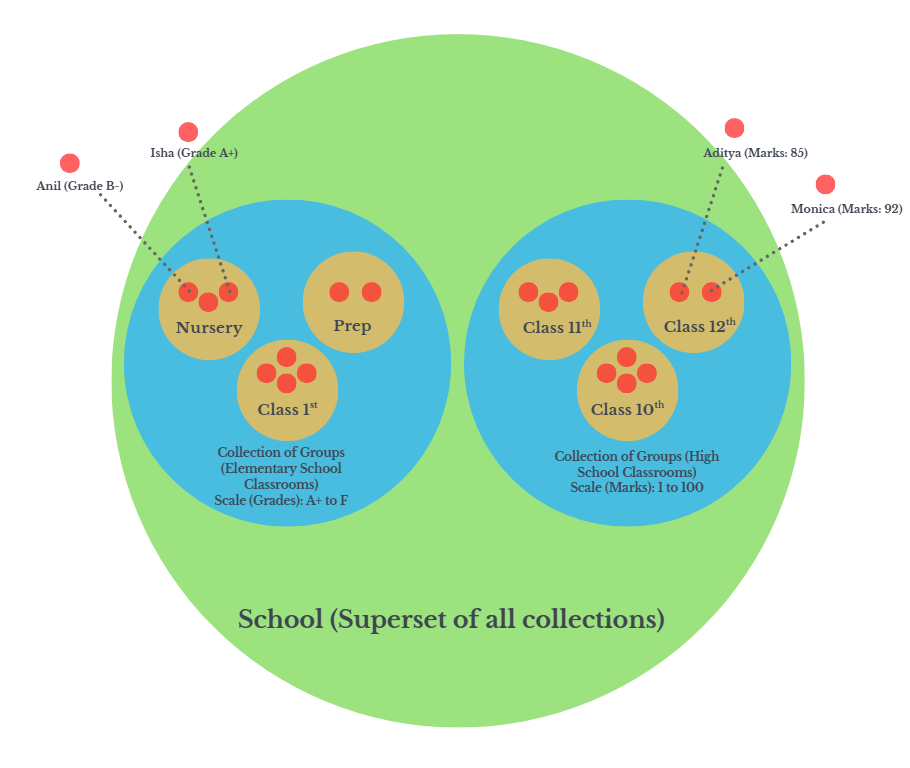
\includegraphics [scale=0.5]{images/superset_collection.png}
    \label{fig:superset-collection}
\end{figure}

The inspiration for the formula came from the idea from \cite{mann1947test}, which uses median to calculate p-value significance. Though, the idea is inspired from their, but applied in terms of assessing performance comparison
for groups having uneven elements, and expanded to create a standardize scale with cross-collection interpretability.

\section{Normalized Group Performance Assessment Formulae}


\begin{equation}
\boxed{
\mathbf{
P_i = \frac{-n_i +  \sum\limits_{j=1}^{n_i} r_j}{n_i \cdot (N - 1)}}
}
\end{equation}
   
\begin{itemize}
    \item \textbf{Ranks}: Sequential ranks assigned to items within and across groups. Tied ranks are averaged out. Note ranks are in ascending order of dominance i.e. rank 1 is the lowest, with rank $N^{th}$ as the highest. This is done to keep symmetry with usage of ranks in other statistics methods such as \cite{mann1947test} etc.
    \item \textbf{$P_i$}: Normalized Performance Measure value of the $i^{th}$ group in the range of [0, 1]
    \item \textbf{$\sum r_j$}: Sum of ranks for group $i$.
    \item \textbf{$n_i$}: number of elements within the $i^{th}$ group
    \item \textbf{$N$}: Total number of elements across all group combined. \hfill \break
    There are \[k = \text{number of groups}, \quad n_i = \text{number of items in each group }\]
    \begin{align}
        \text{N} = \sum\limits_i^k n_i, \quad \text{where N = total number of items}
    \end{align}

\end{itemize}

\subsection{Applications}
This is a list of Applications scenario, the formula was designed for:
\begin{itemize}
	\item \textbf{Psychology}: In Psychology, we have a big arsenal of therapy techniques, all having their own benefits. If, mutually exclusive groups, each group taking a particular therapy, needs to be analyzed which group performed better, and the group sizes are even unequal. Then, Performance Measure Formula can be applied.
    \item \textbf{Educational}: Awarding Best Class Performance in a school, when classes have uneven students, and even different grading scales.
    \item \textbf{Organizational}: To identify best-performing team in the organization, and least-performing, for restructuring and guidance purposes, when number of person per team are uneven, and performance scale at various sector of an organization is different.
   \item \textbf{Business}: Often businesses have economy segment and luxury segment for services and products. Often, just price is not an enough indicator what segment of products fared better. If, a ranking is created, on customer feedback, return on investment, less-after-cost-maintenance, expenses etc. Then, this formula can be used to find the dominant product/services of their business, when there is uneven sale of each product/services sold.
\end{itemize}
There could be applications outside the scope of this paper. But, when designing the formula these above listed applications were being thought of.

\hfill \break
Mathematical derivation, along with its theoretical justification, would be discussed, with its analogous visual intuition where possible. Maxima and Minima, range of normalized performance measure [0, 1], would be proven as well.

\section{Non-normalized Performance}

If you see, the \hyperref[fig:dominance_Understanding]{Figure 2}, is intuitively easy to understand that Group B performance is more dominant, that Group A, simply because Group B occupy the higher ranks, and Group A lower ranks.
\begin{figure}[!htb]
    \caption{Visual intuition of the Performance Measure, Performance: Group B > Group A}
    \centering
    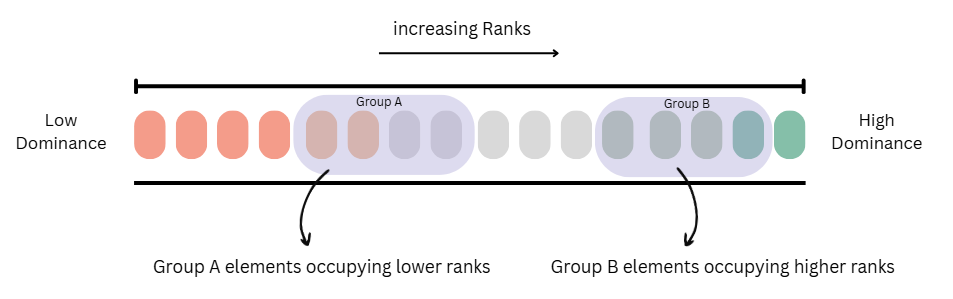
\includegraphics[scale=0.65]{images/dominance-intuition.png}
    \label{fig:dominance_Understanding}
\end{figure}

This non-normalized performance measure, with uneven number of groups is given by:
\begin{equation}
\label{eq:non-normalized}
    p_i^{(non\text{-}normalized)} = w_i \cdot \frac{\sum r_j}{ S_{UDH} }
\end{equation}


\begin{itemize}
	\item Sum of Upper Dominant Half ($S_{UDH}$):
	\begin{align}
		S_{UDH} = \frac{N(N+1)}{2} - \frac{a(a+1)}{2}, \quad a = \lfloor N/2 \rfloor
	\end{align}
	\item Weight Bias ($w_i$):
	\begin{align}
		w_i = \frac{N}{k n_i}
	\end{align}
\end{itemize}

This later non-normalized dominance would be used to derive the normalized version of the formula. Therefore, non-normalized performance derivation would be discussed first.


\subsection{Derivation of Non-normalized Performance}
From, the understanding we gain from \hyperref[fig:dominance_Understanding]{Figure 2}, we can easily, ascertain the local dominance, if we divide the scale into two halves of lower ranks half, and upper rank half. So, the group with ranks in the upper half would have a more prominent or dominant performance. So, we need to figure out what's the ranks of the upper dominant half is.

\subsubsection{Sum of Upper Dominant Half}
\begin{enumerate}
\item{Purpose of UDH}
The \textbf{Upper Dominant Half (UDH)} represents the \textbf{rank sum of the dominant half} of a dataset, providing a benchmark for performance potential in rank-based comparisons.

\item{Total Rank Sum (Full Dataset)}
For a dataset with \textbf{N items}, the \textbf{total rank sum} is the sum of integers from \textbf{1 to N}:
\begin{equation}
S = 1 + 2 + 3 + \ldots + N
\end{equation}
Using the formula for the sum of the first \( N \) integers:
\begin{equation}
S = \frac{N(N + 1)}{2}
\end{equation}

\item{Split the Dataset into Halves}
\begin{itemize}
  \item \( a = \lfloor \frac{N}{2} \rfloor \) represents the size of the \textbf{non-dominant half} (lower half).
  \item The \textbf{dominant upper half} includes the rank from \( a + 1 \) to \(N^{th}\) rank items.
\end{itemize}



\item{Rank Sum of Non-Dominant Half (Lower Half)}
The \textbf{non-dominant half} (lower half) consists of the \textbf{smallest \( a \) ranks}. Its rank sum is:
\begin{equation}
S_{lower} = 1 + 2 + \ldots + a
\end{equation}
Using the formula for sum of integers:
\begin{equation}
S_{lower} = \frac{a(a+1)}{2}
\end{equation}

\item{Rank Sum of Dominant Half (Upper Half)}
The \textbf{Upper Dominant Half} is calculated by subtracting the rank sum of the \textbf{lower half} from the \textbf{total rank sum}:
\begin{equation}
S_{UDH} = S - S_{lower}
\end{equation}
Substituting the formulas:
\begin{equation}
S_{UDH} = \frac{N(N + 1)}{2} - \frac{a(a+1)}{2}
\end{equation}

\item{Final Formula}
\begin{equation}
\label{eq:SUDH}
S_{UDH} = \frac{N(N + 1)}{2} - \frac{a(a+1)}{2}
\end{equation}

\begin{itemize}
  \item \( N \): Total number of items.
  \item \( a \): Size of the lower \textbf{dominant half}, calculated as the floor of half of the net total number of items across all groups, so as to be inclusive of both odd and even count of N items:
  \begin{equation}
  a = \lfloor \frac{N}{2} \rfloor
  \end{equation}
\end{itemize}
\end{enumerate}

\subsubsection*{Non-normalized Performance Formulae (Biased)}
So, to if we compare the ranked sum of the group with the upper dominant half, we can get a numerical understanding of performance measure value
\begin{equation}
\label{eq:p-biased}
    p_i^{(biased)} = \frac{\sum r_j}{ S_{UDH} }
\end{equation}
\begin{itemize}
    \item \textbf{$\sum r_j$}: Sum of ranks for group $i$.
    \item \textbf{$S_{UDH}$}: Sum of Upper Dominant Half
\end{itemize}

As, the formula doesn't take into account weight bias. A high number of items can still occupy lower ranks, but in account of total items in group being large, its ranked sum also gives a higher value. That's why weigh bias was added to adjust this non-normalized performance measure.

\subsubsection*{Weight Bias Derivation}
To derive the weight bias ($w_i$), we first understand, that if all the groups have equal number of items, then $w_i = 1$ i.e. no adjustment needed. That means all the groups have the same number of elements in them. The items expected in each group, can be written as:
\begin{equation}
X_e = \frac{N}{k}
\end{equation}
where:
\begin{itemize}
    \item $X_e$: Expected item count per group.
    \item $k$: Number of groups in collection.
    \item $N$: Total number of items across all groups.
\end{itemize}

So, now we calculate the fractional change needed to reach expected group item
\begin{equation}
 fractional \ change = \frac{X_e - n_i}{n_i}
\end{equation}

If we want to adjust our biased performance, $p_i^{(biased)}$, according to the fractional change, 
then,
\begin{equation}
    p_i^{(unbiased)} = p_i^{(biased)} +  p_i^{(biased)} *  fractional \ change
\end{equation}

in other words, taking $p_i^{(biased)}$ as common, we can rewrite it as
\begin{equation}
\label{eq:p-unbiased}
    p_i^{(unbiased)} = p_i^{(biased)} * (1 +  fractional \ change)
\end{equation}

So, the term needed to adjust from $p_i^{(biased)}$ to $p_i^{(unbiased)}$, can be written as:
\begin{equation}
    w_i = 1 + fractional \ change
\end{equation}

substituting everything we get, the derivation of weight bias:
\begin{equation}\label{eq:weight-bias}
    w_i = \frac{N}{kn_i}
\end{equation}

where:
\begin{itemize}
    \item $w_i$: Weight bias for group $i$.
    \item $n_i$: Number of items in group $i$.
    \item $N$: Total number of items.
    \item $k$: Number of groups.
\end{itemize}

\subsubsection{Final Formula for unbiased (but non\text{-}normalized) Performance Measure}
Therefore, from \hyperref[eq:SUDH]{Equation 12}, \hyperref[eq:p-biased]{Equation 14},  \hyperref[eq:p-unbiased]{Equation 18}, and \hyperref[eq:weight-bias]{Equation 20}

we derived unbiased(but non\text{-}normalized) formulae, as stated in the beginning of the section, in \hyperref[eq:non-normalized]{Equation 3}:
\begin{equation}
	\label{p-non-normalized}
    p_i^{(non\text{-}normalized)} = w_i \cdot \frac{\sum r_j}{ S_{UDH} }
\end{equation}

Note in this research paper, $p_i^{(non\text{-}normalized)}$ = $p_i^{(unbiased)}$ are same, but for standardization sake, we will use $p_i^{(non\text{-}normalized)}$ moving forward.

\section{Normalized Performance Measure}

The unbiased and non-normalized formulae, is needed to be normalized, for to satisfy these following criteria:
\begin{itemize}
	\item Explicitly provides a meaningful zero baseline for dominance measures.
	\item Performance scores become standardized, allowing direct comparisons across multiple studies or scenarios
\end{itemize}
Given by:
\begin{equation}
	\boxed{
		\mathbf{
			P_i = \frac{-n_i +  \sum\limits_{j=1}^{n_i} r_j}{n_i \cdot (N - 1)}}
	}
\end{equation}
This formulae is the conclusion of whole paper, which is named Normalized Performance Measure.

\subsection{Derivation of Normalized Performance Measure}

For normalizing the performance we will find the theoretical minima and maxima of non-normalized performance. 

\subsubsection{Minima of Non-normalized Performance Measure}

Thus, we start with the assumption that the net total number of items across all groups is even (odd case would be taken later in the paper), then it is safe to assume that:

\begin{align*}
	a = \frac{N}{2}
\end{align*}

Thus, the lower and upper halves would be explicitly:
\[
\left[1, \frac{N}{2}\right] \quad \text{and} \quad \left[\frac{N}{2}+1, N\right]
\]

Simplifying for $S_{UDH}$ when N is even, we get:

\begin{equation}
	\label{eq:even-SUDH}
	S_{UDH} = \frac{N(3N + 2)}{8}
\end{equation}


We aim to minimize the non-normalized measure $p_i^{(non\text{-}normalized)}$ defined as:
\begin{equation}
	p_i^{(non\text{-}normalized)} = w_i \cdot \frac{\sum r_j}{ S_{UDH} }
\end{equation}

Substituting everything into our non-normalized measure equation, we get:

\begin{align*}
	p_i^{(non\text{-}normalized)} = \frac{8}{k(3N + 2)}\cdot \frac{\sum r_j}{n_i}
\end{align*}

As, 
\begin{equation}
	\frac{8}{k(3N + 2)} = Constant
\end{equation}

The minima, depends on $\frac{\sum r_j}{n_i}$. And, for this to be low $\sum r_j$ should be low. That means $r_j$ have to occupy the lowest ranks such as 1, 2, 3,... so on. We can rewrite $\frac{\sum r_j}{n_i}$ in this format below:

\begin{equation}
	 = \frac{\sum r_j}{n_i} = \frac{\frac{n_i}{2}(1+n_i)}{n_i} = \frac{1}{2} \cdot n_i + \frac{1}{2}
\end{equation}

As this is a linearly increasing line equation with a positive slope ($y = mx + C$), minima of $\frac{\sum r_j}{n_i}$ occurs when $n_i = 1$, as $n_i$ is a natural number and can't be zero or negative, hence, substituting $n_i = 1$, we get, $\frac{\sum r_j}{n_i} = \frac{1}{2} + \frac{1}{2} = 1$, hence  $\frac{\sum r_j}{n_i} = 1 $

Therefore minima of Non-normalized measure is:
\begin{equation}
	\label{eq:minima}
	p_i^{(min, \, non\text{-}normalized)} = \frac{8}{k(3N + 2)}
\end{equation}

\subsubsection{Maxima of Non-normalized Performance Measure}
Similar to minima, being:

\begin{align*}
	p_i^{(non\text{-}normalized)} = \frac{8}{k(3N + 2)}\cdot \frac{\sum r_j}{n_i}
\end{align*}

As, 
\begin{equation}
	\frac{8}{k(3N + 2)} = Constant
\end{equation}

Maxima depends on $\frac{\sum r_j}{n_i}$, which needs to be maximized. Therefore, $r_j$ will contain higher ranks, such as N, N-1, N-2,...,k. So, The lowest rank in this arithmetic series can contain is k. Because, there are k groups, that means, each will have at least one element, occupying the lowest ranks, to maximize $\frac{\sum r_j}{n_i}$. That means, first group will contain rank 1, second group will contain rank 2, so on..., and the $k^{th}$ group will have the rest of the elements from rank $k^{th}$ to $N^{th}$ element which we are trying to maximize. Then $\sum r_j$, can be expanded to:
\begin{equation}
	\frac{(N-k+1)(N+k)}{2}
\end{equation}
As, $n_i$ are the number of elements in the group which is equal to $N-k+1$, then simplifying $\frac{\sum r_j}{n_i}$, we get:
\begin{equation}
	\frac{N+k}{2}
\end{equation}

Now to maximize, we can substitute k with N, as k are number of groups, and the max number of groups would be equal to total number of items in the collection, where each group has just one element.
hence maximum value comes out to be:
\begin{equation}
	\frac{\sum r_j}{n_i} = N
\end{equation}
 
Therefore maxima of Non-normalized Measure is:
\begin{equation}
	\label{eq:maxima}
	p_i^{(max, \, non\text{-}normalized)} = \frac{8N}{k(3N + 2)}
\end{equation}

\subsubsection{Final formualae of Normalized Performance Measure}
Normalized Performance measure would be given by:
\begin{equation}
	\label{eq:normalized-simpler}
	P_i = \frac{p_i^{(non\text{-}normalized)} - p_i^{(min, \, non\text{-}normalized)}}{p_i^{(max, \, non\text{-}normalized)} - p_i^{(min, \, non\text{-}normalized)}}
\end{equation}

Now substituting their corresponding value from \hyperref[p-non-normalized]{Equation 21},  
 \hyperref[eq:even-SUDH]{Equation 23}, \hyperref[eq:minima]{Equation 27} and \hyperref[eq:maxima]{Equation 32}, and simplifying, we get the final form of Normalized Performance Measure:
\begin{equation}
	\boxed{
		\mathbf{
			P_i = \frac{-n_i +  \sum\limits_{j=1}^{n_i} r_j}{n_i \cdot (N - 1)}}
	}
\end{equation}
\begin{itemize}
	\item \textbf{$P_i$}: Normalized Performance Measure value of the $i^{th}$ group in the range of [0, 1]
	\item \textbf{$\sum r_j$}: Sum of ranks for group $i$.
	\item \textbf{$n_i$}: number of elements within the $i^{th}$ group
	\item \textbf{$N$}: Total number of elements across all group combined. \hfill \break
\end{itemize}

\subsubsection{Normalized Performance Measure (Scenario: N is odd)}
We will not go in thorough detail, but the Normalized performance measure formula is same. Because the, Sum of Upper Dominant half ($S_{UDH}$), maxima and minima just differ slightly in nature. But, as these terms occur in the numerator and denominator, they cancel each other out. And, \textbf{the Normalized Performance Measure remains unchanged}. Just, to be complete, we will just list down the equations, which result in the same formula as above.

As, N is odd, where $N^{(min)} = 3$, because there has to be minimum of two groups, therefore, we will take,
\begin{align*}
	a = \frac{N-1}{2}
\end{align*}

Thus, the lower and upper halves would be explicitly:
\[
\left[1, \frac{N-1}{2}\right] \quad \text{and} \quad \left[\frac{N+1}{2}, N\right]
\]

when N is odd:

\begin{equation}
	\label{eq:even-SUDH-odd}
	S_{UDH} = \frac{(N+1)(3N+1)}{8}
\end{equation}

\begin{equation}
	\label{eq:minima-odd}
	p_i^{(min, \, non\text{-}normalized)} = \frac{8N}{k (N+1)(3N+1)}
\end{equation}

\begin{equation}
	\label{eq:maxima-odd}
	p_i^{(max, \, non\text{-}normalized)} = \frac{8N^2}{k (N+1)(3N+1)}
\end{equation}

substituting their corresponding value in \hyperref[eq:normalized-simpler]{Equation 33} from \hyperref[p-non-normalized]{Equation 21},  
\hyperref[eq:even-SUDH-odd]{Equation 35}, \hyperref[eq:minima-odd]{Equation 36} and \hyperref[eq:maxima-odd]{Equation 37}, and simplifying, we get the final form of Normalized Performance Measure (same as when N is even):
\begin{equation}
	\boxed{
		\mathbf{
			P_i = \frac{-n_i +  \sum\limits_{j=1}^{n_i} r_j}{n_i \cdot (N - 1)}}
	}
\end{equation}


\subsubsection{Range of Normalized Performance Measure}
Minima of $P_i = 0$, which means is the least dominant performance, that means in the entire collection they have a group containing, one element with Rank 1. Mathematically, $p_i^{(non\text{-}normalized)} =  p_i^{(min, \, non\text{-}normalized)}$, thus, putting the value in the \hyperref[eq:normalized-simpler]{Equation 33}, we get:
\begin{equation}
	P_i^{(min)} = \frac{p_i^{(min, \, non\text{-}normalized)} - p_i^{(min, \, non\text{-}normalized)}}{p_i^{(max, \, non\text{-}normalized)} - p_i^{(min, \, non\text{-}normalized)}} = 0
\end{equation}

Similarly,
Maxima of $P_i^{(max)} = 1$, which means is the most dominant performance, that means in the entire collection they have a group containing, one element with Rank $N^{th}$, the highest ranked element possible. Mathematically, $p_i^{(non\text{-}normalized)} =  p_i^{(max, \, non\text{-}normalized)}$, thus, putting the value in the \hyperref[eq:normalized-simpler]{Equation 33}, we get:
\begin{equation}
	P_i^{(max)} = \frac{p_i^{(max, \, non\text{-}normalized)} - p_i^{(min, \, non\text{-}normalized)}}{p_i^{(max, \, non\text{-}normalized)} - p_i^{(min, \, non\text{-}normalized)}} = 1
\end{equation}

Therefore, the range of normalized performance measure is [0,1]


\section{Validation}
All mathematical and numerical validation scripts, as well as the full manuscript source, are available in the GitHub repository \cite{silentkarmi2025normalized}. See the repository's folder structure and README for details on specific files and validation types.

\subsection{Mathematical Validation: Theoretical Derivation via SymPy Library in Python}
To, validate all manual work, the formula also has been derived through mathematical coding via SymPy library using Python Language (a open source replacement tool for Mathematica), written inside a Jupyter Notebook.

A snippet of the code is hereby attached: \hyperref[code:snippet_odd_performance_measure]{Python (SymPy) Code Snippet}. This snippet is for: When N is odd, Mathematical Derivation of Normalized Performance Measure.

 	\label{code:snippet_odd_performance_measure}
\begin{mintedbox}{python}
	# code snippet
	
	display("N is odd then,")
	
	a = (n - 1)/2
	s_udh = n*(n+1)/2 - a*(a+1)/2
	display("S_UDH = ",simplify(s_udh))
	
	p_i = w_i * sigma_r_j / s_udh
	display("p_i_normalized = ", simplify(p_i))
	
	p_i_min = p_i.subs({n_i:1}) # number of elements = 1
	p_i_min = p_i_min.doit()
	p_i_min = p_i_min.subs({r[1]:1}) # containing one element rank = 1
	display("p_i_minima_non-normalized = ",simplify(p_i_min))
	
	p_i_max = p_i.subs({n_i:1}) # number of elements = 1
	p_i_max = p_i_max.doit()
	p_i_max = p_i_max.subs({r[1]:n}) # containing one element rank = Nth
	display("p_i_maxima_non-normalized = ",simplify(p_i_max))
	
	P_i = (p_i - p_i_min)/(p_i_max - p_i_min)
	display("Normalized Performance Measure, P_i = ", factor(simplify(P_i)))
\end{mintedbox}

\hyperref[fig:output-mathematical-validation]{Figure 3} shows the output of the Snippet Code
\begin{figure}[!htb]
	\caption{Output: Mathematical Derivation of Normalized Performance Measure via SymPy}
	\centering
	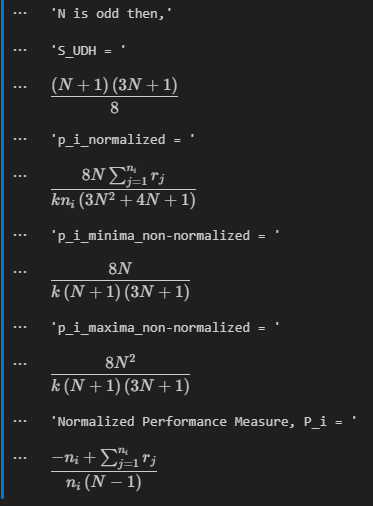
\includegraphics [scale=1]{images/output-mathematical-validation.png}
	\label{fig:output-mathematical-validation}
\end{figure}

\subsection{Numerical Validation: Range of Normalized Performance Measure}
We have mathematically and theoretically have proven the range to [0,1].
Zero means the group has single element with Rank 1 element, lowest performance measure value possible.
And, one means the group has single element with Rank $N^th$ element, highest performance measure value possible.
Any combination of elements in the group will be in the range of [0,1].

We have used this simple numerical example to validate, where value is same with their rank.
\begin{table}[htbp]
	\centering
	\caption{Example used for Validation of Range for Normalized Performance Measure}
	\begin{tabular}{llcc}
		\toprule
		\textbf{Group} & \textbf{Member Value} & \textbf{Rank} & \textbf{Normalized Performance Measure} \\
		\midrule
		I     & 1   & 1   & 0.0 \\
		\midrule
		\multirow{9}{*}{II} 
		& 2   & 2   & \multirow{9}{*}{0.5} \\
		& 3   & 3   &  \\
		& 4   & 4   &  \\
		& 5   & 5   &  \\
		& 6   & 6   &  \\
		& 7   & 7   &  \\
		& 8   & 8   &  \\
		& 9   & 9   &  \\
		& 10  & 10  &  \\
		\midrule
		III   & 11  & 11  & 1.0 \\
		\bottomrule
	\end{tabular}
	\label{tab:validation}
\end{table}


This is numerically validated via Python code, by applying the formulae discussed in the research paper, the code snippet is attached below:


\begin{mintedbox}{python}
	def setPerformanceMeasureValue(self):
	"""Calculates the normalized performance value, using the formula in the research paper
	"""
	ni = self.getElementCount()
	sigma_ri = self.getRankedGroupSum()
	n = self.parent.netTotalItemsInCollection
	k = self.parent.getNumberOfGroups()
	self.performanceMeasureValue = (-ni + sigma_ri)/(ni*(n-1))
\end{mintedbox}

\hyperref[fig:output-numerical-validation-minima-maxima]{Figure 4} shows the output of Maxima and Minima Validation.
\begin{figure}[!htbp]
	\caption{Output: Numerical Validation of Range for Normalized Performance Measure via Python}
	\centering
	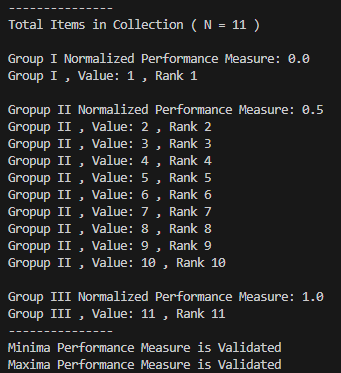
\includegraphics [scale=1]{images/output-validation-minima-maxima.png}
	\label{fig:output-numerical-validation-minima-maxima}
\end{figure}


\section{Detailed Example of Dominance Method}

\subsection{Validation of Results}
\begin{itemize}
	\item cross-validation from a different method
\end{itemize}
\printbibliography
\appendix
\end{document}

%% 
%% Copyright (C) 2019 by Daniel A. Weiss <daniel.weiss.led at gmail.com>
%% 
%% This work may be distributed and/or modified under the
%% conditions of the LaTeX Project Public License (LPPL), either
%% version 1.3c of this license or (at your option) any later
%% version.  The latest version of this license is in the file:
%% 
%% http://www.latex-project.org/lppl.txt
%% 
%% Users may freely modify these files without permission, as long as the
%% copyright line and this statement are maintained intact.
%% 
%% This work is not endorsed by, affiliated with, or probably even known
%% by, the American Psychological Association.
%% 
%% This work is "maintained" (as per LPPL maintenance status) by
%% Daniel A. Weiss.
%% 
%% This work consists of the file  apa7.dtx
%% and the derived files           apa7.ins,
%%                                 apa7.cls,
%%                                 apa7.pdf,
%%                                 README,
%%                                 APA7american.txt,
%%                                 APA7british.txt,
%%                                 APA7dutch.txt,
%%                                 APA7english.txt,
%%                                 APA7german.txt,
%%                                 APA7ngerman.txt,
%%                                 APA7greek.txt,
%%                                 APA7czech.txt,
%%                                 APA7turkish.txt,
%%                                 APA7endfloat.cfg,
%%                                 Figure1.pdf,
%%                                 shortsample.tex,
%%                                 longsample.tex, and
%%                                 bibliography.bib.
%% 
%%
%% End of file `./samples/longsample.tex'.
